\section{Perils of disregard}

Consider the following scenarios: 1) Based on recent input from the public, the Department of Transportation (DOT)
of a certain city is considering implementing a new parking policy that discourages parking in the Central Business
District and therefore would encourage the use of more active transportation modes such as walking or biking.
2) A certain DOT is considering implementing a Streetcar system to incentivize more transit oriented development in a certain region. 

When thinking about these two "policy" proposals (funding the Streetcar system in the second case),
it could that the DOT (or any other agency) in question ran analyses (either based on meticulous 
modeling or anectodal evidence) that allowed them to deduce that implementing such policies would 
directly result in their desired output or achieve their desired goal.
This inherently assumes the causal relationship between the policy and the final output 
(implementing the new parking policy will increase the share of active transportation modes in 
CBDs and funding the streetcar system will generate more transit oriented developments).
Moreover, these analyses - and conclusions from such analyses - of the impact of the proposed 
policies are also based on a certain belief of how the the world or the system works. 
However, in many instances (insert references to policies etc..) such belief of structure of the 
system is not made clear; we only hear about the policy and its most downstream impact. 
Such depiction of proposed policies maintains an obscure representation (at least to the knowledge 
of the average person) of the system and the interactions between its intermediate elements.

Directed Acyclic Graphs (DAGs) otherwise known as causal graphs allow one to clearly represent 
one's assumptions about the problem at hand.
DAGs have been used in fields ranging from epidemiology, scheduling, and network structures 
and have shown to be extremely useful. 

DAGs could show to be very useful in addressing policy questions (in our case transportation policy questions).
Brathwaite & Walker \citet{brathwaite_2018_causal} have illustrated an example of how DAGs can be used to answer such questions.
Brathwaite & Walker, however, have not showed an empirical application of how using DAGs can result in 
different model estimates when compared to traditional methods of modeling.
In this section, we will show how to structurally approach demand modeling problems while paying close 
attention to the data generating process and the causal structure of how people make choices.
We approach this exercise by building up on work from Brathwaite's and Walker's work by going through 
the motions of empirical exercise exemplifying a simplified problem.
We want to note that this example is for illustrative reasons and that it does not reflect the complexities 
usually accompanying a transportation choice modeling exercise.
Let's assume that a company wants to reduce its workforce carbon footprint by moving its employees closer to campus.
We would like to model the travel mode choice of these workers based on a dataset from Brathwaite & Walker /citet{brathwaite-asymmetric}.
This dataset comes from the 2012 California Household Travel Survey (CHTS).
It contains 4004 home-based school or work tours made by approximately 3850 individuals in the Bay area. 
Readers interested in a more detailed description of the dataset can refer to Brathwaite & Walker /citet{brathwaite-asymmetric}. 
We would like to remind readers that our goal in this section is to only show how one's beliefs and assumptions about the data generation
process affect estimates from the outcome model and that controlling for intermediate variables of 
some policy variable of interest in a causal graph,
we do not succeed at recovering the true causal parameters of the variable of interest.
For purposes of this exercise, we take the Multinomial Logit model defined in Brathwaite & Walker /citet{brathwaite-asymmetric} as the true outcome generating process.

The systematic portion of the the multinomial logit model from Bratwhaite and Walker /citet{brathwaite-asymmetric} is specified as follows:

TODO: convert the following equations.

U_da = $beta_{time_drive}$ * tavel_time + $beta_{cost_per_distance_da}$*cost_per_distance_da + $beta_{autos_ld_auto}$*number_of_autos_per_ld
U_sr2 = $ASC_{sr2}$ + $beta_{time_drive}$ * tavel_time + $beta_{cost_per_distance_sr2}$*cost_per_distance_sr2 + $beta_{autos_ld_auto}$*number_of_autos_per_ld + $beta_{cross_bay}$*cross_bay_tour + $beta_{hhsize}$ * household_size + $beta_{n_kids_hh}$ * number_of_kids_hh
U_sr2 = $ASC_{sr3+}$ + $beta_{time_drive}$ * tavel_time + $beta_{cost_per_distance_sr3+}$*cost_per_distance_sr3+ + $beta_{autos_ld_auto}$*number_of_autos_per_ld + $beta_{cross_bay}$*cross_bay_tour + $beta_{hhsize}$ * household_size + $beta_{n_kids_hh}$ * number_of_kids_hh
U_WTW = $ASC_{WTW}$ + $beta_{travel_time_transit}$ *travel_time + $beta_{travel_cost}$ * tavel_cost
U_DTW = $ASC_{DTW}$ + $beta_{travel_time_transit}$ *travel_time + $beta_{travel_cost}$ * tavel_cost
U_WTD = $ASC_{WTD}$ + $beta_{travel_time_transit}$ *travel_time + $beta_{travel_cost}$ * tavel_cost

We achieve our goal through a simulation exercise as follows:

1. We generate a causal graph where we assume that all explanatory variables are observed and that there 
is no no structural relationship between any of them. 
We simulate data based on this graph and then simulate outcomes based on parameters from a well-defined 
mode choice model using a Multinomial Logit (MNL) choice model described in Brathwaite & Walker /citet{brathwaite-asymmetric}.
We will then apply the do-operator [reference if not mentioned earlier] perturb the travel distance 
variable to emulate the company's decision to move its employees closer to campus.
We will then predict outcomes based on the mode choice model.

2. We generate a different causal graph based on different assumptions of how explanatory variables influence and interact with each other.
We estimate the relationships outlined in this causal graph between different nodes based on the data at hand.
We simulate "upstream" nodes not affected by any other nodes in the causal graph and use the estimated relationships 
between the explanatory variables to estimate the remaining explanatory variables.
We then use the choice model from step 1 to simulate outcome choices based on this new dataset.
We move to apply the do-operator to perturb the variable of interest (in our case travel distance) to replicate the intervention 
resulting from a policy changing travel distance, and use the estimated relationships between the explanatory 
variables in the causal graph to simulate all the explanatory variables in the causal graph.
We use the estimated choice model to produce outcomes based on the newly estimated data. 

We repeat this simulation process numerous times and recover the probabilities that each individual chooses a certain mode. 
In this exercise, we focus on the probability of choosing car-centric modes (Drive alone, Shared ride with another 
person, and a shared ride with two or more individuals).
We compute the difference in probabilities generated by the different models based on different data generating processes.

Figure \ref{fig:IND_GRAPH} shows the causal graph where all explanatory variables are independent of each other for each utility equation.

\begin{figure}
   \centering
   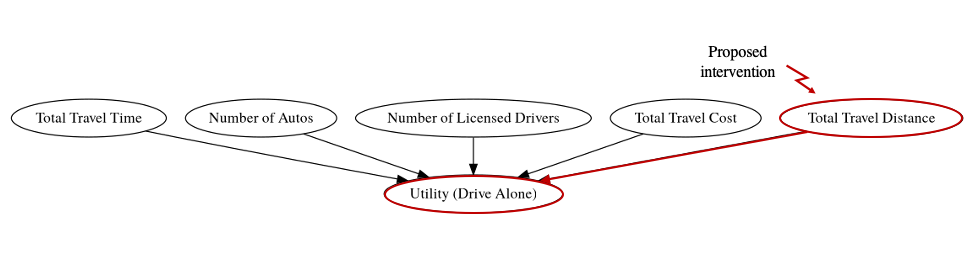
\includegraphics[width=0.5\textwidth]{Independent_graph.png}
   \caption{Causal Graph with Independent Covariates}
   \label{fig:IND_GRAPH}
\end{figure}

The variables shown in the graph are assumed to be all of the explanatory variables needed to estimate the outcome and are based 
on the specification of the MNL model outlined in Brathwaite & Walker [reference].
We can describe the variables as follows:
- Total travel distance: is the total travel distance for individual i and mode j, for all available modes for individual i during trip t of tour l.
- Total travel cost: is the travel cost in dollars for individual i and mode j, for all available modes for individual i during trip t of tour l.
- Total travel time: is the travel time in minutes for individual i and mode j, for all available modes for individual i during trip t tour l.
- Number of autos: is the number of automobiles owned by individual i's Household
- Number of licensed drivers: is the number of licensed drives in individual i's household.
- Number of kids: is the number of kids (specify age?) in individual i's household.
- Cross-bay trip: is a binary variable indicating whether the trip t for individual 1 is a cross-bay trip.

Similarly, Figure \ref{fig:DA_causal_2} through \ref{fig:BIKE_causal_2} illustrate the causal graphs with "interacting" explanatory variables.
\begin{figure}
   \centering
   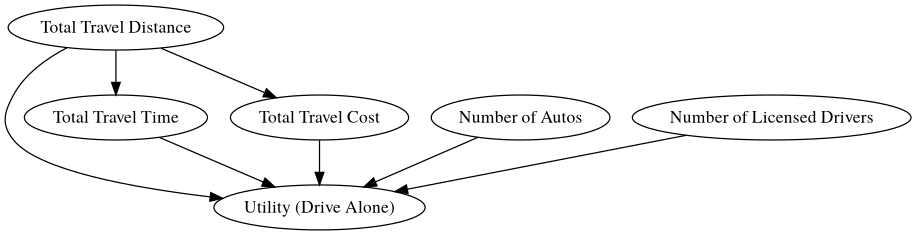
\includegraphics[width=0.5\textwidth]{DA_interacting_graph.png}
   \caption{Causal Graph for the Drive Alone Utility Function}
   \label{fig:DA_causal_2}
\end{figure}

\begin{figure}
   \centering
   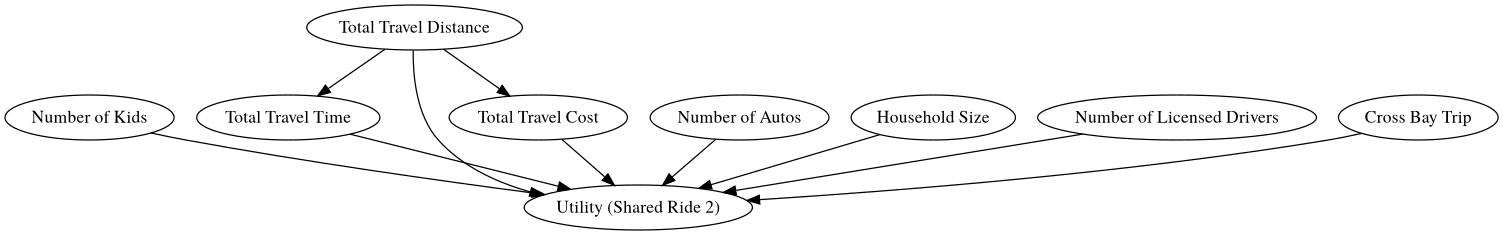
\includegraphics[width=0.5\textwidth]{SR2_interacting_graph.png}
   \caption{Causal Graph for the Shared Ride 2 Utility Function}
   \label{fig:SR2_causal_2}
\end{figure}

\begin{figure}
   \centering
   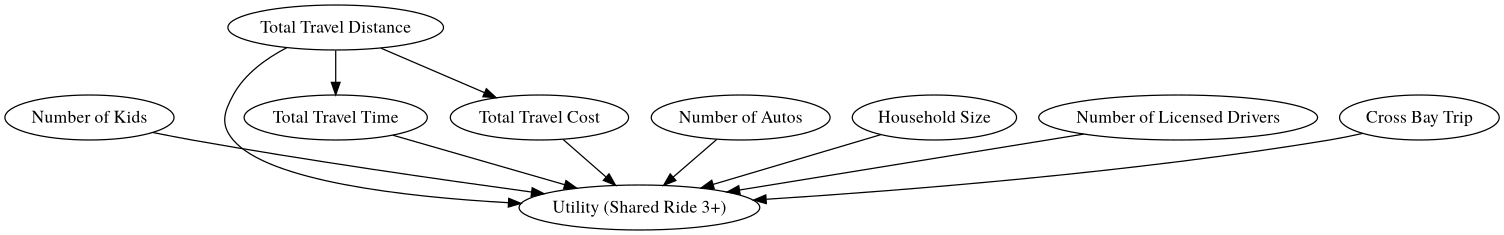
\includegraphics[width=0.5\textwidth]{SR3_interacting_graph.png}
   \caption{Causal Graph for the Shared Ride 3+ Utility Function}
   \label{fig:SR3_causal_2}
\end{figure}

\begin{figure}
   \centering
   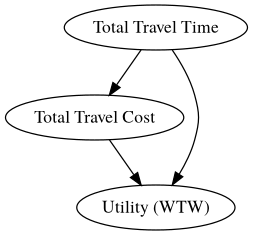
\includegraphics[width=0.5\textwidth]{WTW_interacting_graph.png}
   \caption{Causal Graph for the Walk-Transit-Walk Utility Function}
   \label{fig:WTW_causal_2}
\end{figure}

\begin{figure}
   \centering
   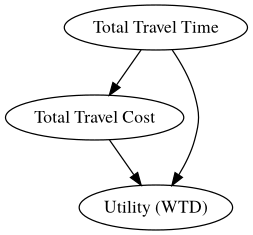
\includegraphics[width=0.5\textwidth]{WTD_interacting_graph.png}
   \caption{Causal Graph for the Walk-Transit-Drive Utility Function}
   \label{fig:WTD_causal_2}
\end{figure}

\begin{figure}
   \centering
   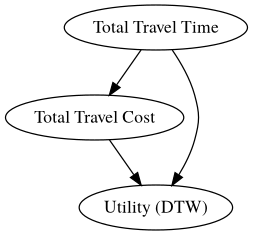
\includegraphics[width=0.5\textwidth]{DTW_interacting_graph.png}
   \caption{Causal Graph for the Drive-Transit-Walk Utility Function}
   \label{fig:DTW_causal_2}
\end{figure}

\begin{figure}
   \centering
   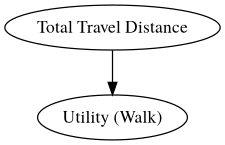
\includegraphics[width=0.5\textwidth]{WALK_interacting_graph.png}
   \caption{Causal Graph for the Shared Ride 3+ Utility Function}
   \label{fig:WALK_causal_2}
\end{figure}

\begin{figure}
   \centering
   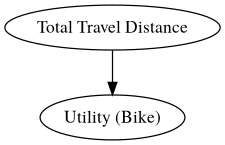
\includegraphics[width=0.5\textwidth]{BIKE_interacting_graph.png}
   \caption{Causal Graph for the Bike Utility Function}
   \label{fig:BIKE_causal_2}
\end{figure}

Each of these graphs is based on the utility function of each respective mode in the multinomial logit model estimated in Brathwaite and Walker /citet{brathwaite-asymmetric}.

We then plot histograms of the computed differences between the average probability of an individual 
in our sample choosing a car centric mode before and after implementing a policy or intervention
aimed at reducing travel distance.
These differences are plotted under the two different assumptions about the data generating process illustrated in the causal graphs above.
Figure \ref{fig:histogram_probability} highlights the bias between the estimated probability of an average individual choosing a car centric mode.
This difference shows the importance of considering the data generating process when estimating transportation demand models aiming to forecast the impact of proposed policies.

\begin{figure}
   \centering
   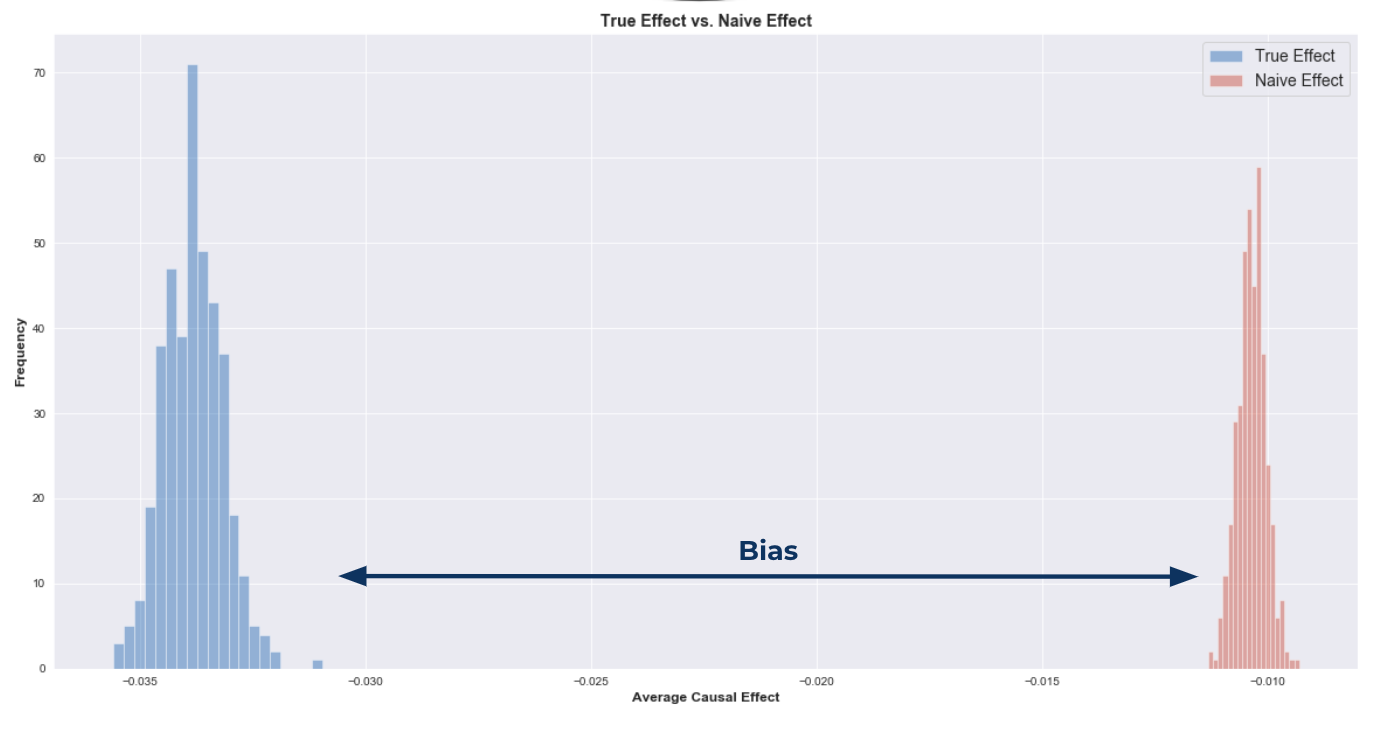
\includegraphics[width=0.5\textwidth]{histogram_selection_on_obs.png}
   \caption{Histograms of the probability of choosing Car Centric Modes under Different Data Generating processes.}
   \label{fig:histogram_probability}
\end{figure}

The data generating process might not be easily distinguishable in the majority of situations, mainly due to the complexity of the real world.
Therefore, constructing a causal graph that represents the data generating process as much as possible is not an easy task.
This chapter explores other topics related to this matter, including some guidance on how to build and test causal graphs representing the researchers beliefs about the data generating process.
\blindtext[2]

\blindtext[2]